\documentclass[border={0.1cm 0.1cm 0.1cm 0.1cm}]{standalone}  %E,S,W,N

\usepackage{amssymb}
\usepackage{amsmath}
\usepackage{tikz}
\usetikzlibrary{decorations.pathreplacing}	%for brackets

\begin{document}
	
	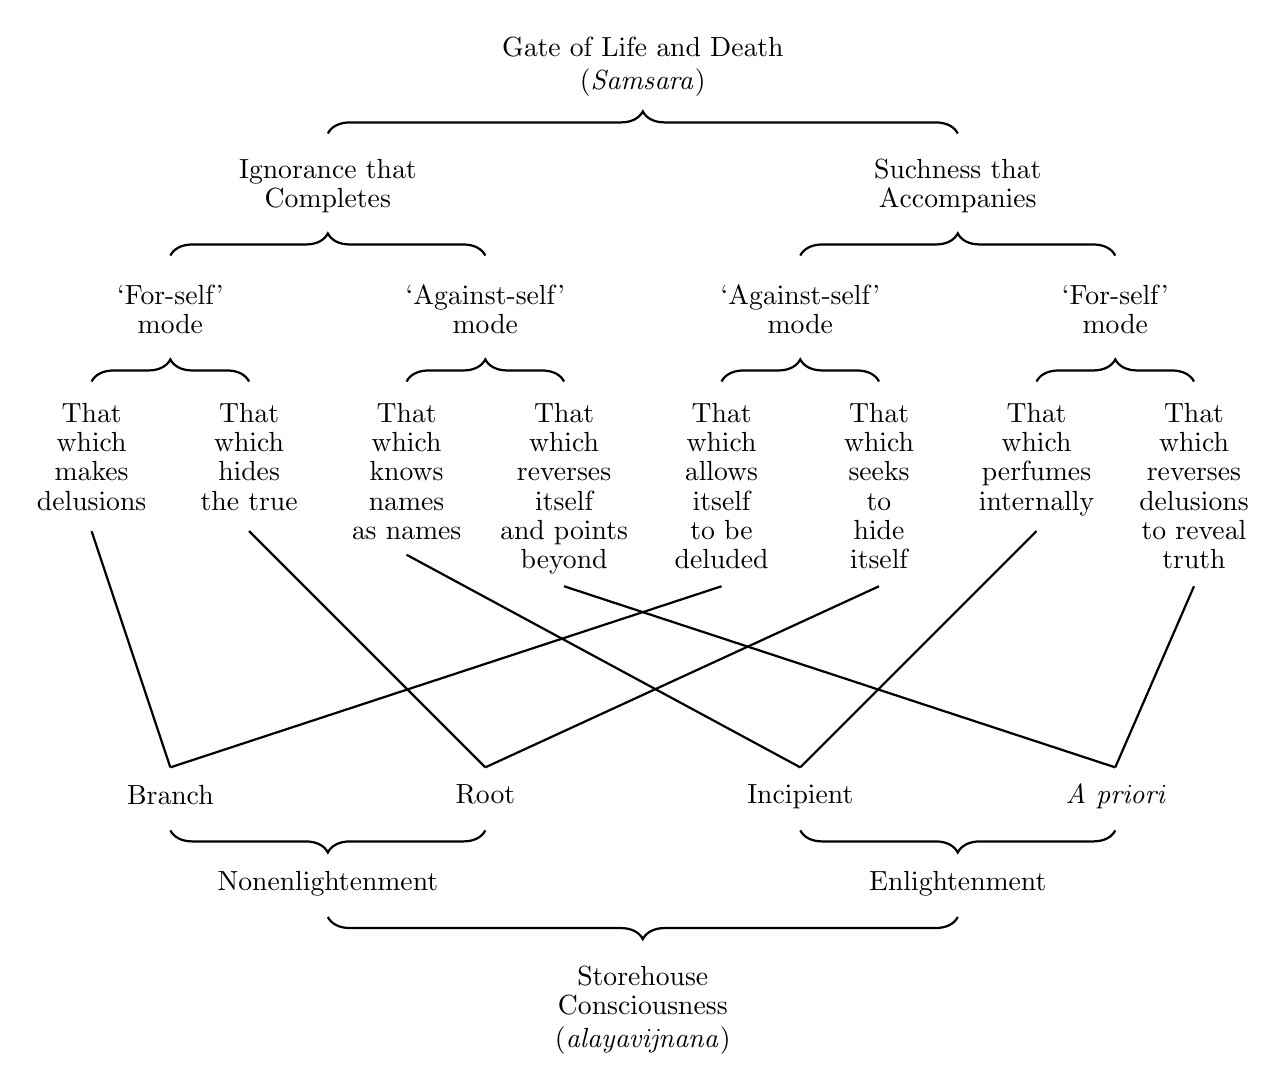
\begin{tikzpicture}	
	\node[align=center] at (0,-0.1) {Gate of Life and Death \\ (\textit{Samsara})};
	\draw[decorate,decoration={brace,amplitude=8pt},thick] (-4,-0.95)--(4,-0.95);
	
	\node[align=center,below] at (-4,-1.15) {Ignorance that \\[-0.5mm] Completes};
	\node[align=center,below] at (4,-1.15) {Suchness that \\[-0.5mm] Accompanies};
	
	\draw[decorate,decoration={brace,amplitude=8pt},thick] (-6,-2.5)--(-2,-2.5);
	\draw[decorate,decoration={brace,amplitude=8pt},thick] (2,-2.5)--(6,-2.5);
	
	\node[align=center,below] at (-6,-2.75) {`For-self' \\[-0.5mm] mode};
	\node[align=center,below] at (-2,-2.75) {`Against-self' \\[-0.5mm] mode};
	%
	\node[align=center,below] at (2,-2.75) {`Against-self' \\[-0.5mm] mode};
	\node[align=center,below] at (6,-2.75) {`For-self' \\[-0.5mm] mode};
	
	\draw[decorate,decoration={brace,amplitude=8pt},thick] (-7,-4.1)--(-5,-4.1);
	\node[align=center,below] at (-7,-4.25) {That \\[-0.5mm] which \\[-0.5mm] makes \\[-0.5mm] delusions};
	\node[align=center,below] at (-5,-4.25) {That \\[-0.5mm] which \\[-0.5mm] hides \\[-0.5mm] the true};
	
	\draw[decorate,decoration={brace,amplitude=8pt},thick] (-3,-4.1)--(-1,-4.1);
	\node[align=center,below] at (-3,-4.25) {That \\[-0.5mm] which \\[-0.5mm] knows \\[-0.5mm] names \\[-0.5mm] as names};
	\node[align=center,below] at (-1,-4.25) {That \\[-0.5mm] which \\[-0.5mm] reverses \\[-0.5mm] itself \\[-0.5mm] and points \\[-0.5mm] beyond};
	
	\draw[decorate,decoration={brace,amplitude=8pt},thick] (1,-4.1)--(3,-4.1);
	\node[align=center,below] at (1,-4.25) {That \\[-0.5mm] which \\[-0.5mm] allows \\[-0.5mm] itself \\[-0.5mm] to be \\[-0.5mm] deluded};
	\node[align=center,below] at (3,-4.25) {That \\[-0.5mm] which \\[-0.5mm] seeks \\[-0.5mm] to \\[-0.5mm] hide \\[-0.5mm] itself};
	
	\draw[decorate,decoration={brace,amplitude=8pt},thick] (5,-4.1)--(7,-4.1);
	\node[align=center,below] at (5,-4.25) {That \\[-0.5mm] which \\[-0.5mm] perfumes \\[-0.5mm] internally};
	\node[align=center,below] at (7,-4.25) {That \\[-0.5mm] which \\[-0.5mm] reverses \\[-0.5mm] delusions \\[-0.5mm] to reveal \\[-0.5mm] truth};
	
	\node[align=center,below] at (-6,-9.1) {Branch};
	\node[align=center,below] at (-2,-9.1) {Root};
	\node[align=center,below] at ( 2,-9.1) {Incipient};
	\node[align=center,below] at ( 6,-9.1) {\itshape A priori};
	
	\draw[thick] (-6,-9)--(-7,-6);	\draw[thick] (-6,-9)--(1,-6.7);	%Branch
	\draw[thick] (-2,-9)--(-5,-6);	\draw[thick] (-2,-9)--(3,-6.7);	%Root
	\draw[thick] ( 2,-9)--(-3,-6.3);	\draw[thick] ( 2,-9)--(5,-6);	%Incipient
	\draw[thick] ( 6,-9)--(-1,-6.7);		\draw[thick] ( 6,-9)--(7,-6.7);	%A Priori
	
	\draw[decorate,decoration={brace,amplitude=8pt},thick] (-2,-9.8)--(-6,-9.8);
	\draw[decorate,decoration={brace,amplitude=8pt},thick] (6,-9.8)--(2,-9.8);
	\node[align=center,below] at (-4,-10.2) {Nonenlightenment};
	\node[align=center,below] at ( 4,-10.2) {Enlightenment};
	\draw[decorate,decoration={brace,amplitude=8pt},thick] (4,-10.9)--(-4,-10.9);
	\node[align=center,below] at (0,-11.4) {Storehouse \\[-0.5mm] Consciousness \\ (\textit{alayavijnana})};
	\end{tikzpicture}
	
\end{document}